\documentclass[main.tex]{subfiles}

\begin{document}
\subsubsection{Sizes of Local Group galaxies}
Like we did for constellations last week, we'll work in pairs and then as a class to construct a scale model of the Local Group, the small cluster of galaxies which the Milky Way is a member of. 

Astronomers have determined the distances to the galaxies in our neighbourhood through a variety of methods. We have also measured their angular sizes, which we will use to estimate their actual sizes.
\begin{enumerate}
\item Working in pairs, go to the Galaxy Data Sign-up link for this lab on Moodle and fill out your names at the next available galaxy.
\item Using a scale of 1 m for 500,000 light-years (2 m for 1 million (1,000,000) ly), have one person stand at a distance from the whiteboard corresponding to the galaxy distance.
\item Have the other person stand at the whiteboard and mark out a width that corresponds to \SI{2}{\degree} of angular width, as seen by the first person. (This is about the width of your thumbnail with your arm fully extended in front of you.) 

Record this width in centimetres: \rule{2cm}{.15mm}

If your galaxy is at a distance that is too close for you to be able to stretch out your arm fully, move 3 times farther from the board, and then divide your final size by 3.

\item Trade places and repeat, then average your results.
\item Using this scale, mark out the size of your galaxy as estimated from its observed angular size $\alpha$, e.g. if your galaxy is \SI{0.1}{\degree} across, it extends 0.1/2 of the width you have marked out. Use the following formula:
\begin{equation*}
\frac{\alpha}{\SI{2}{\degree}} \times \text{width in centimetres} = \rule{2cm}{.15mm}\ \si{\cm}
\end{equation*}
At this scale, the Milky Way, which has a diameter of about 90,000 ly, is about 18 cm in diameter.

\item Using the same scale of 500,000 light-years per 1 m, i.e. 5,000 light-years per 1 cm, estimate the true size of your galaxy. Fill out the data for your galaxy below.
\begin{table}[h!]
%\caption{default}
\begin{center}
\begin{tabular}{|c|c|c|c|c|}\hline
No. & Galaxy Name & Distance (light-years) & Angular diameter ($\alpha$/\si{\degree}) & Diameter (light-years)\\\hline
&&&&\\
&&&&\\\hline
\end{tabular}
\end{center}
\label{tab:gal}
\end{table}
%\vspace{-20pt}
\item Using colours to denote galaxy type according to the table, make a model of your galaxy as follows.
\begin{table}[h!]
\begin{center}
\begin{tabular}{|c|c|c|}\hline
E/Sph & S (a-m) & Irr \\\hline
Yellow & Green & Blue\\\hline
\end{tabular}
\end{center}
\label{tab:galcol}
\end{table}
%\vspace{-20pt}

If your galaxy is small enough to fit on a small piece of paper, draw it as a circle of the correct size and colour it in with the right colour. If not, get a piece of paper of the right colour and cut out a circle of the correct size to attach to your paper.
\end{enumerate}

The colours also simulate how the galaxies appear. E (elliptical)/Sph (spherical) galaxies, mostly dwarf (dE, dSph), mostly have older yellow stars. S (spiral) galaxies have older yellow stars in the center and star formation making newer, bluer stars in the disk. Irr (irregular) galaxies usually have lots of star formation, which makes new, bluer stars.

\subsubsection{Positions of Local Group galaxies}
Galaxies in the Local Group mostly lie on a fairly flat plane, so we have assigned them an azimuth according to the direction they lie from the Milky Way. Now, we'll model their positions in space.
\begin{enumerate}
\item Your galaxy has an azimuth associated with it. Find the direction of your galaxy relative to the Milky Way. Use the position of the Milky Way we have put up and azimuth values we have marked.
\item In that direction, go out the corresponding distance of your galaxy from the Milky Way, and put it down. Remember that the scale is 500,000 light-years per metre.
\item Mark the position in the diagram.
\end{enumerate}
\begin{figure}[htbp]
\begin{center}
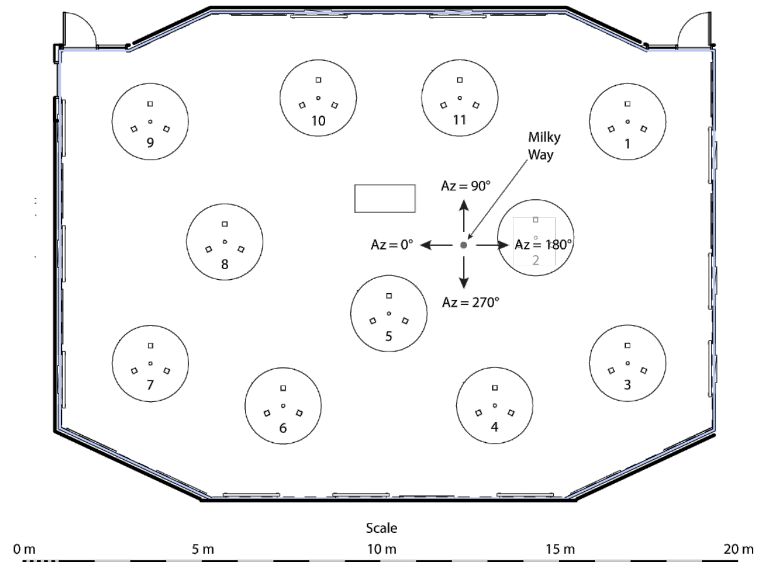
\includegraphics[width=\textwidth]{galclass.png}
%\caption{default}
\label{fig:galclass}
\end{center}
\end{figure}
 
\subsubsection{Moodle Lab Quiz}
Go to the section for this lab on the Moodle page and complete the End-of-Lab Quiz.

Be sure to complete the post-lab survey on Moodle before the deadline. Credit is awarded only for completion, not for correctness.
\end{document}